\documentclass[]{elsarticle} %review=doublespace preprint=single 5p=2 column
%%% Begin My package additions %%%%%%%%%%%%%%%%%%%
\usepackage[hyphens]{url}

  \journal{European Commission Press Release Database} % Sets Journal name


\usepackage{lineno} % add
\providecommand{\tightlist}{%
  \setlength{\itemsep}{0pt}\setlength{\parskip}{0pt}}

\bibliographystyle{elsarticle-harv}
\biboptions{sort&compress} % For natbib
\usepackage{graphicx}
\usepackage{booktabs} % book-quality tables
%%%%%%%%%%%%%%%% end my additions to header

\usepackage[T1]{fontenc}
\usepackage{lmodern}
\usepackage{amssymb,amsmath}
\usepackage{ifxetex,ifluatex}
\usepackage{fixltx2e} % provides \textsubscript
% use upquote if available, for straight quotes in verbatim environments
\IfFileExists{upquote.sty}{\usepackage{upquote}}{}
\ifnum 0\ifxetex 1\fi\ifluatex 1\fi=0 % if pdftex
  \usepackage[utf8]{inputenc}
\else % if luatex or xelatex
  \usepackage{fontspec}
  \ifxetex
    \usepackage{xltxtra,xunicode}
  \fi
  \defaultfontfeatures{Mapping=tex-text,Scale=MatchLowercase}
  \newcommand{\euro}{€}
\fi
% use microtype if available
\IfFileExists{microtype.sty}{\usepackage{microtype}}{}
\usepackage{longtable}
\usepackage{graphicx}
% We will generate all images so they have a width \maxwidth. This means
% that they will get their normal width if they fit onto the page, but
% are scaled down if they would overflow the margins.
\makeatletter
\def\maxwidth{\ifdim\Gin@nat@width>\linewidth\linewidth
\else\Gin@nat@width\fi}
\makeatother
\let\Oldincludegraphics\includegraphics
\renewcommand{\includegraphics}[1]{\Oldincludegraphics[width=\maxwidth]{#1}}
\ifxetex
  \usepackage[setpagesize=false, % page size defined by xetex
              unicode=false, % unicode breaks when used with xetex
              xetex]{hyperref}
\else
  \usepackage[unicode=true]{hyperref}
\fi
\hypersetup{breaklinks=true,
            bookmarks=true,
            pdfauthor={},
            pdftitle={Is welfare state the priority? Refugees flow through Europe and their target countries},
            colorlinks=false,
            urlcolor=blue,
            linkcolor=magenta,
            pdfborder={0 0 0}}
\urlstyle{same}  % don't use monospace font for urls

\setcounter{secnumdepth}{0}
% Pandoc toggle for numbering sections (defaults to be off)
\setcounter{secnumdepth}{0}
% Pandoc header



\begin{document}
\begin{frontmatter}

  \title{Is welfare state the priority? Refugees flow through Europe and their
target countries}
    \author[Universidade Federal de Pernambuco - UFPE]{Stephanie Moura de Oliveira\corref{c1}}
   \ead{stephaniemoura.cp@gmail.com} 
   \cortext[c1]{Corresponding Author}
      \address[Universidade Federal de Pernambuco - UFPE]{Universidade Federal de Pernambuco}
  
  \begin{abstract}
  Over the past years, the civil war in Syria and all the danger that
  accompanies it, caused a great number of syrian nationals to leave their
  homes and their nation with the main objective of surviving the attacks
  suffered daily in the country. The Syrian refugees are crossing european
  borders for the past years and this is causing a malaise between the war
  refugees and nationals of the countries that receive them. In this
  paper, we will evaluate whether the welfare state and quality of life
  indexes of European countries have been attractive enough for Syrian
  nationals who have left their country to spend time or establish their
  permanent residence, or if only the prospect of having a peaceful space
  and safe to live for a period of time and then return to their country
  of origin is enough. In this paper we analyze the intentions of the
  refugees when seeking an asylum and the connexion between variables that
  express quality of life and the entry and asylum of syrian refugees on
  2011 and 2015, years that represent the biggest influxes of syrians in
  Europe, after the Arab Spring and during the war.
  \end{abstract}
  
 \end{frontmatter}

\section{Introduction and Theory}\label{introduction-and-theory}

Countries with higher rates of Welfare State lead to more syrian asylum
applications? With the advance of the refugee crisis and a consequent
increase on the number of people in need of a new homeland to call its
own, European countries have reshaped their immigration policies in
order to accommodate (or not) the growing number of refugee requests.

The country whose internal conflict has caused more nationals to leave
its territory was Syria, since after the start of the Arab Spring in
2010 and a series of popular protests in the country, that progressed to
a violent armed revolt, influenced by other protests in the Arab world.

The conflict shows itself in two fronts: one compound by oppositors of
the President Bashar Al-Assad, that claims to be struggling to oust his
power and then later install a more democratic leadership in the
country; and the other composed by Assad and its government, who claims
to be only fighting armed terrorists who aim to destabilize the country.
Over the years, this war with an initial political cause, turned itself
into a ``power struggle'', also embracing aspects with sectarian and
religious natures, that lead to the emergence of many factions that now
fight against each other and the government.

In the middle of this conflict, many civilians found themselves in the
middle of bombings, and more than five million Syrians would have tried
to escape the fighting, most of them seeking refuge abroad. The conflict
generated a huge migratory wave of Syrians and Arabs towards Europe. It
is the largest migratory wave and consequent humanitarian crisis faced
by Europe since World War II. According to the Vice-President of the
European Commission, Frans Timmermans, it is a ``world crisis that needs
an European answer'' (Timmermans 2018).

This migratory flow reached critical levels throughout 2015, with an
exponential increase (hundreds of thousands of people) trying to enter
Europe and applying for asylum. These people flew away of their
countries due to wars, conflicts, hunger, religious intolerance,
terrible climate change, human rights violations, hopelessness and
others, and adding to all this, a massive action of intimidation,
violence and oppression carried out by groups that control illegal
trafficking exploited these totally vulnerable migrants (Duarte-Plon
2015).

But why did so many migrants seek Europe to take refuge instead of
seeking asylum in other Middle Eastern or Asian countries closer to
their country of origin? The answer to this can maybe be found on a
definition of Welfare State: ``A welfare state is a state in which
organized power is deliberately used (through politics and
administration) in an effort to modify the play of the market forces in
at least three directions - first, by guaranteeing individuals and
families a minimum income irrespective of the market value of their work
or their property; - second, by narrowing the extent of insecurity by
enabling individuals and families to meet certain ``social
contingencies'' (for example, sickness, old age and unemployment) which
lead otherwise to individual and family crisis; and - third, by ensuring
that all citizens without distinction of status or class are offered the
best standards available in relation to a certain agreed range of social
services.'' (Briggs 1961)

The sociologist T. H. Marshall described the modern welfare state as a
distinctive combination of democracy, welfare and capitalism. As a type
of mixed economy, the welfare state funds the governmental institutions
for healthcare and education along with direct benefits paid to
individual citizens. Modern welfare states include Germany, France,
Belgium and the Netherlands, as well as the Nordic countries, which
employ a system known as the Nordic Model. The various implementations
of the welfare state fall into three categories: (i) social democratic,
(ii) conservative, and (iii) liberal. (Marshall 1992)

That said, this paper tries to enlight if countries with a higher
Welfare State attract more requests for refuge, these being preferred by
refugees from Syria. This analysis is important to help the
understanding of the movement trends of refugees if they are looking for
countries with a higher quality of life or just a country where they can
allocate themselves to escape the conflicts. This may also lead to
explanations about the preference of refugees to remain in the place of
refuge after the conflict ends or to return to their homeland.

The hypothesis that this work will try to falsify is that the number of
requests for refugees from Syria to countries in Europe are influenced
by the level of Welfare State of these countries.

\section{Methodology}\label{methodology}

This paper will use as methodology for data analysis the R software,
with which a linear regression will be performed in order to evaluate by
country the number of requests for refuge by Syrian citizens. The years
to be analyzed are 2011 and 2015, with the aim of analyzing before and
after the refugee crisis, after the beginning of the Arab Spring. The
objective was to analyze the situation of refugees in a more recent
scenario after the onset of the crisis, but because of the lack of data
available from more recent years.

For the analysis, two databases will be used, the UNHCR Population
Statistics Database, which contains data on asylum and refuge
applications for several countries in the world over several years by
citizens from different countries. From this database will be taken the
dependent variable on the number of asylum requests from Syrians in
European countries, the ``Applied'' variable. In addition to this, the
Quality of Government (QOG) standard database of January 2018 will be
used, the most complete and up-to-date of QoG's databases. From this
database will be taken the independent variables that characterize the
welfare state. Variables with greater data availability were searched
for the largest number of countries in the analyzed years. Thus, the
variables chosen were ``Health'', ``Equitable Education'' and ``Public
Service''. Besides these, the variable ``Political Rights'' is used as
control because it is an indicator of democracy and of the country's
development then it wants to see the effect of public services
controlling for this variable of political development of the country.
The effect of not including it can be an overestimation of the effect of
the other variable.

\section{Operationalizing the
Variables}\label{operationalizing-the-variables}

The research question that we try to answer is:

\textbf{Countries with higher rates of Welfare State lead to more syrian
asylum applications?}

In this paper, an analysis about the number of refuge requests from
Syria in european countries is made, regarding their level of Welfare.
Trying to understand the movement trends of refugees, four variables
from the Quality of Government database (QOG Standard - Jan - 2018), and
one variable from the United Nations High Commissioner for Refugees
(UNHCR Population Statistics - Resettlement) is used in this paper with
the object of explaining the most recent refugees movements from Syria
to European Countries, trying to understand if the number of refuge
requests has some relation with the welfare state level of the countries
to which the requests were directed.

That said, it's important to enlight which were the variables used in
the paper. The independent variables selected for this paper were
extracted from the QOG Basic Database. And these variables were:

\begin{itemize}
\tightlist
\item
  \textbf{ffp\_ps} (using various algorithms, this variable is converted
  into a score representing the significance of the public services for
  each country. The smaller, the better);
\item
  \textbf{bs\_ee} (refers to equitable education and the qualitative
  indicators reflect the evaluations provided by more than 100 experts
  responding to the SGI's survey of the state of affairs in various
  policy areas throughout the OECD and EU. For these indicators, the
  rating scale ranges from 1 (worst) to 10 (best);
\item
  \textbf{bs\_h} (refers to the quality of the health system. The
  qualitative indicators reflect the evaluations provided by more than
  100 experts responding to the SGI's survey of the state of affairs in
  various policy areas throughout the OECD and EU. For these indicators,
  the rating scale ranges from 1 (worst) to 10 (best).);
\item
  Above these, the \textbf{fh\_pr} is a variable that refers to
  political rights, and in this paper is used as a control variable (the
  specific list of rights considered varies over the years. Countries
  are graded between 1 (most free) and 7 (least free)). The
  \textbf{fh\_pr} variable is used as control because it is an indicator
  of democracy and of the country's development then wants to see the
  effect of public services controlling for this variable of political
  development of the country. The effect of not including it can be an
  overestimation of the effect of the other variable.
\end{itemize}

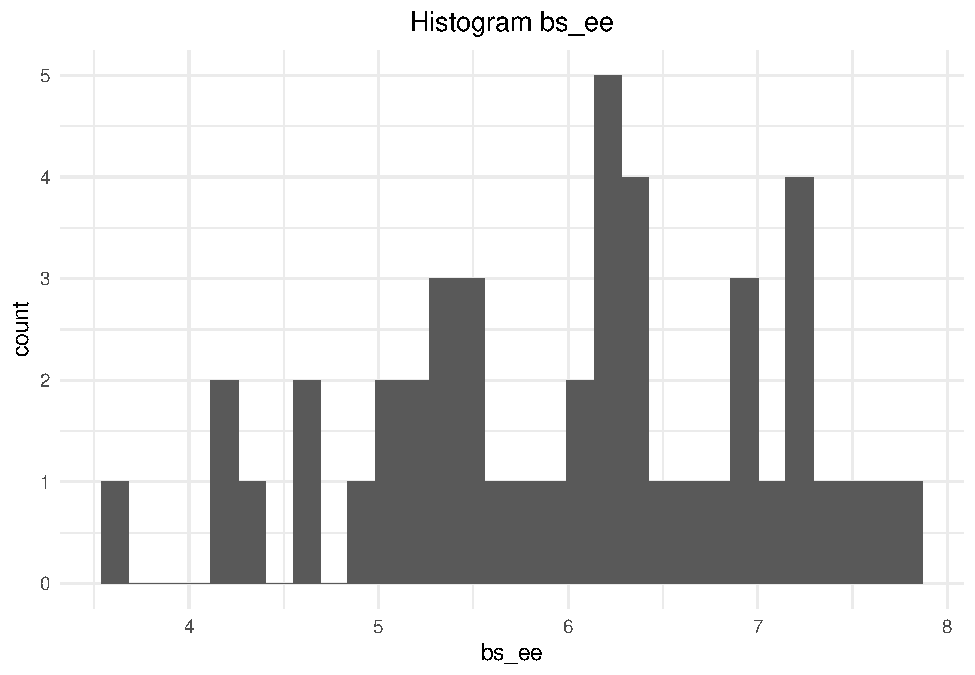
\includegraphics{stephanie-moura-rmarkdown-tf-ad-ufpe-2018_files/figure-latex/ggplot_variables1-1.pdf}

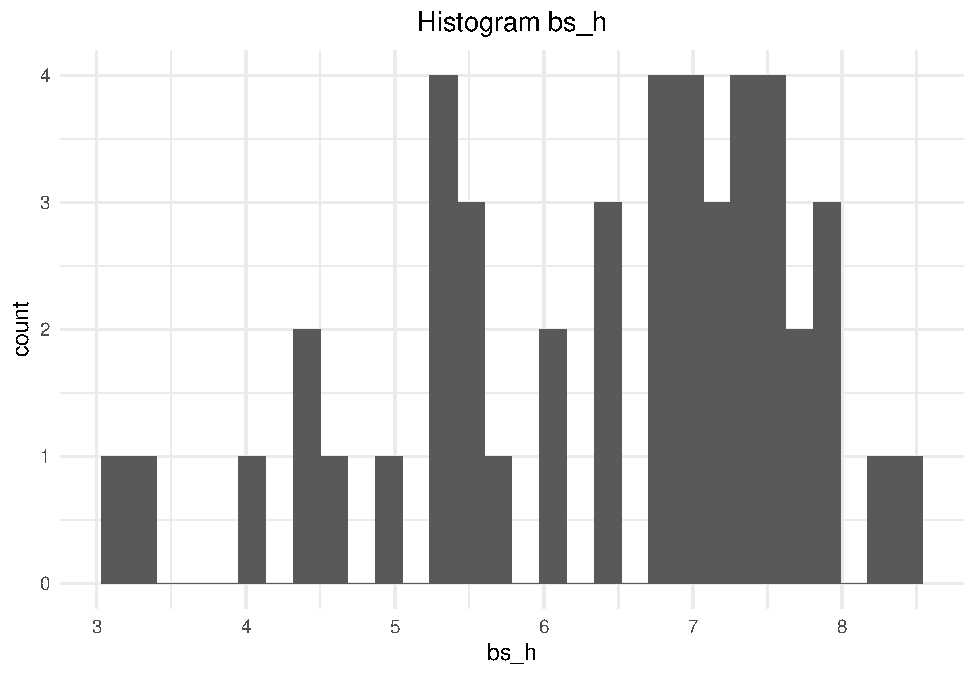
\includegraphics{stephanie-moura-rmarkdown-tf-ad-ufpe-2018_files/figure-latex/ggplot_variables2-1.pdf}

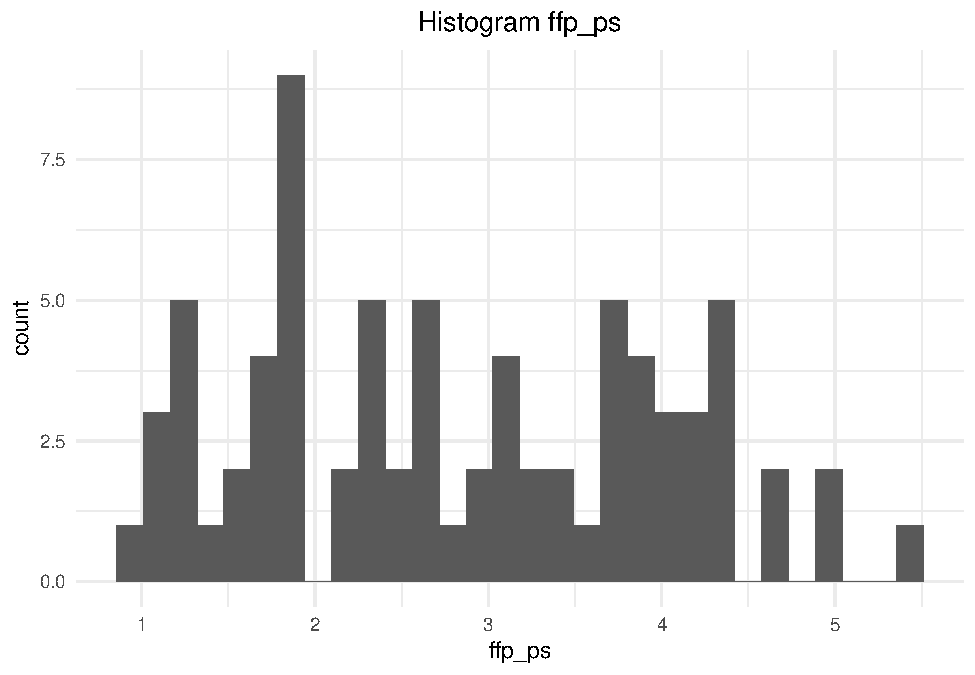
\includegraphics{stephanie-moura-rmarkdown-tf-ad-ufpe-2018_files/figure-latex/ggplot_variables3-1.pdf}

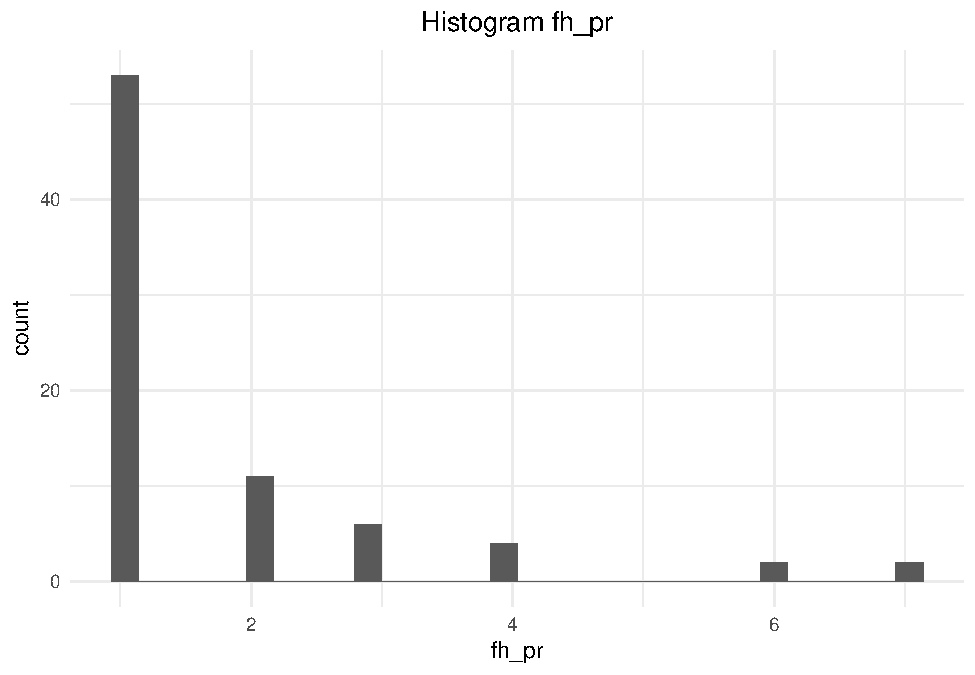
\includegraphics{stephanie-moura-rmarkdown-tf-ad-ufpe-2018_files/figure-latex/ggplot_variables4-1.pdf}

The dependent variable ``Applied'' was extracted from the UNHCR
database, which shows the number of refuge requests on each year
analyzed, from Syrian citizens for each country on the analysis. The
descriptive statistics of the independent variable ``Applied'' will then
be presented. The ``Applied'' variable presented a mean of
`5105.8333333.

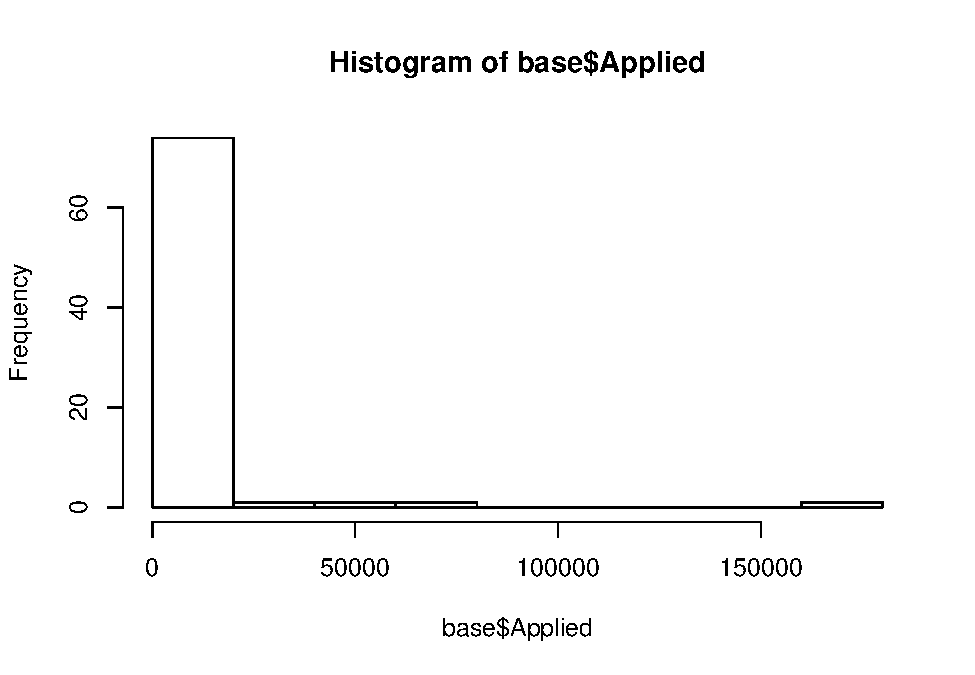
\includegraphics{stephanie-moura-rmarkdown-tf-ad-ufpe-2018_files/figure-latex/histo_1-1.pdf}

After the selection of the variables, tests with the logarithmic
transformation are made. It's possible to notice that the distribution
is almost normal. The log is used once it's assumed that the
distribution of the variable has a bias, therefore, one of the
extremities has a long tail, and once it's measured as correlation or
regression, it can be greatly influenced by peak distribution, outliers,
among others. The transformation can reduce the bias effect. After the
logatithmic transformation, and with the variables ready for the
analysis, it is going to be used linear regression models, to process
and present the results (summary). The linear regressions were made
separately with the objective of not reducing too much the cases since
the bs\_ee and bs\_h variables are present in different countries than
the ``ffp\_ps'' and ``fh\_pr''. Then it's decided to set up four linear
regression models, one for the political rights and public services
variables in 2011, one for these variables in 2015, and one for the
equitable education, health and political rights variables in 2011 and
other for these variables in 2015.

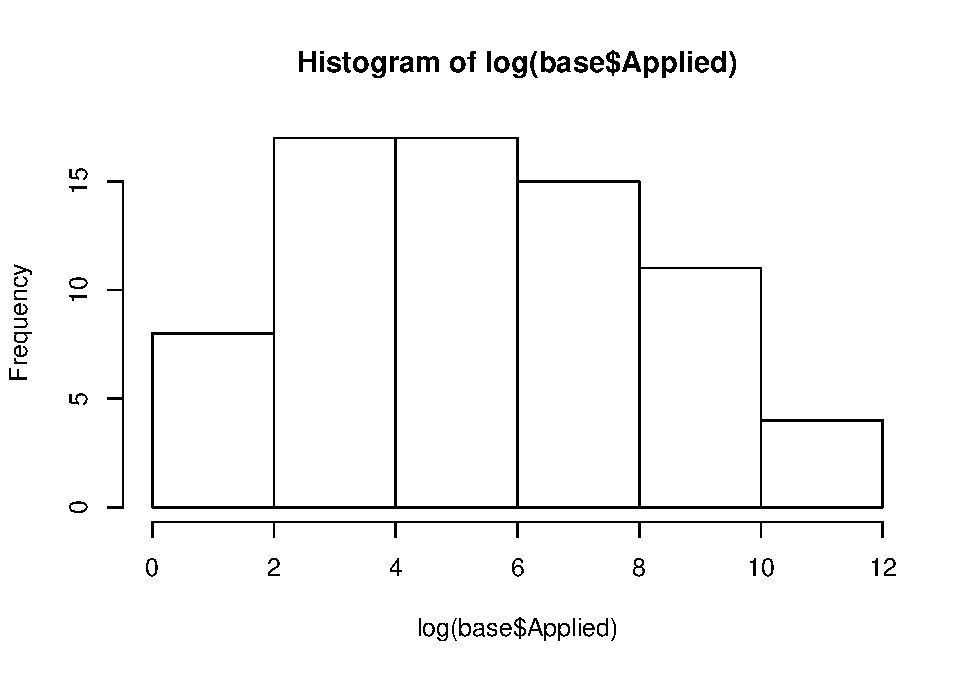
\includegraphics{stephanie-moura-rmarkdown-tf-ad-ufpe-2018_files/figure-latex/histo_2-1.pdf}

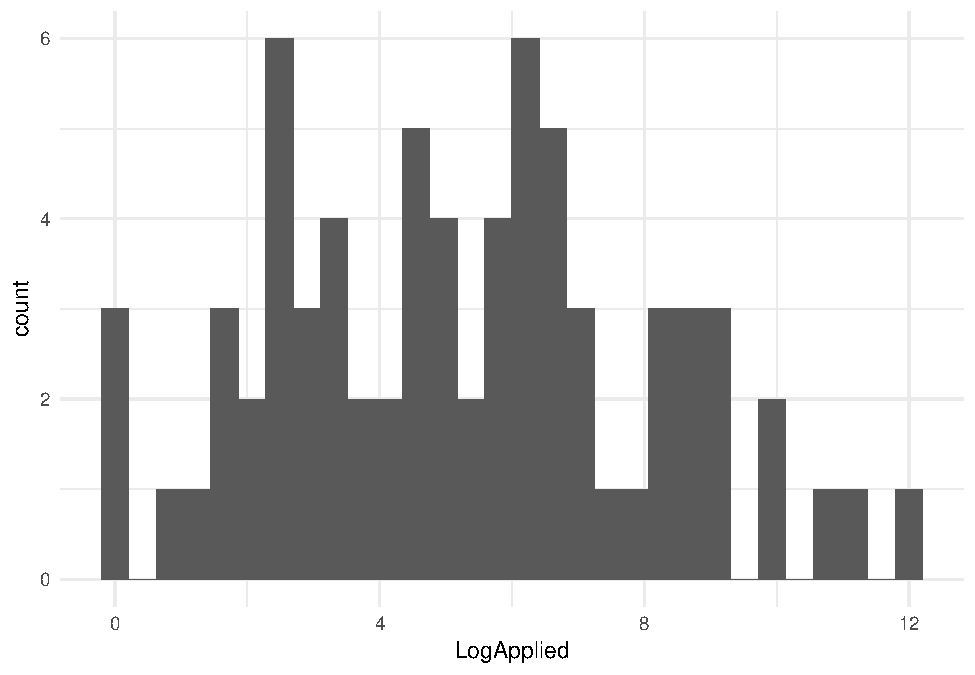
\includegraphics{stephanie-moura-rmarkdown-tf-ad-ufpe-2018_files/figure-latex/base_log-1.pdf}

The four models have the objective of explaining in as much detail as
possible the motivations that led the Syrian refugees to apply for
asylum in the European countries analyzed in the years 2011 and 2015.
Then it's made a code to produce a table with the regression results.
Will be a table in a text type, with the title ``Model Results'', in an
American Journal of Political Science Style, including p-values. After
that, dispersion graphics indicating the relationship between the
variables and add regression line are made.

First we check the association, in a scatter plot, between the variables
``Health'' and ``Applied''. The correlation result between the variables
was low, 0.27, and positive, indicating that the association between the
variables is imprecise but that to some extent, when one variable
increases, the other decreases, being proportional.

As an additional analysis, we constructed graphs of association between
the variables, seeking to identify possible non-linear relationships.

Concerning the graphic that associates the variables ``number of refuge
requests'' and ``public services'', we can see that as public services
increase, the number of requests for refuge decreases, in 2011.

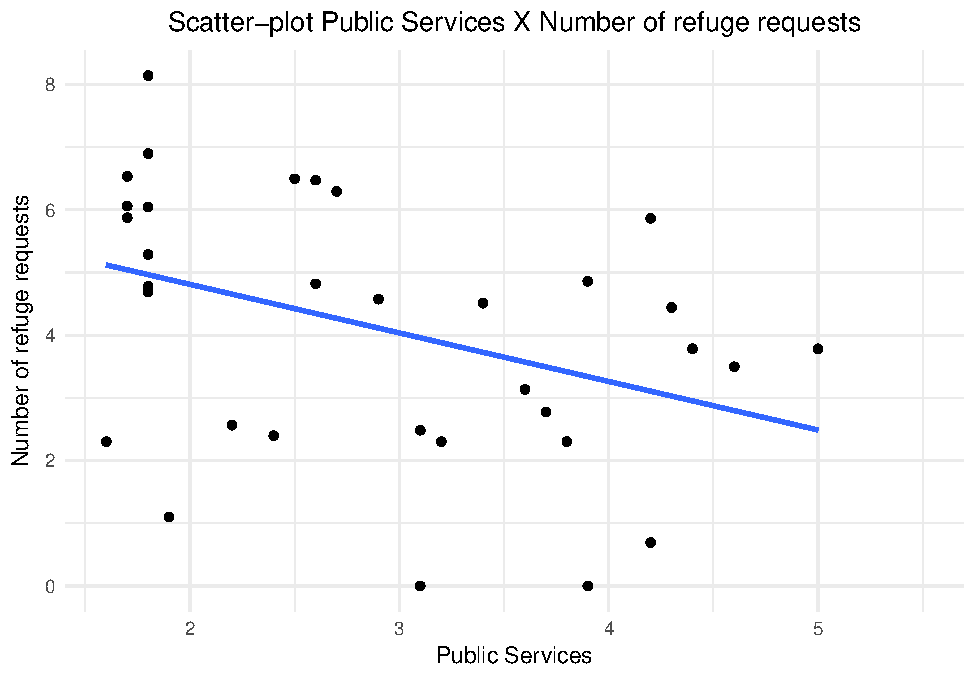
\includegraphics{stephanie-moura-rmarkdown-tf-ad-ufpe-2018_files/figure-latex/model_1_1-1.pdf}

Concerning the graph that associates the variables ``number of refuge
requests'' and ``Health and equitable education'', we can see that as
the Health and Equitable education index increases, the number of
refugee requests increases, in 2011.

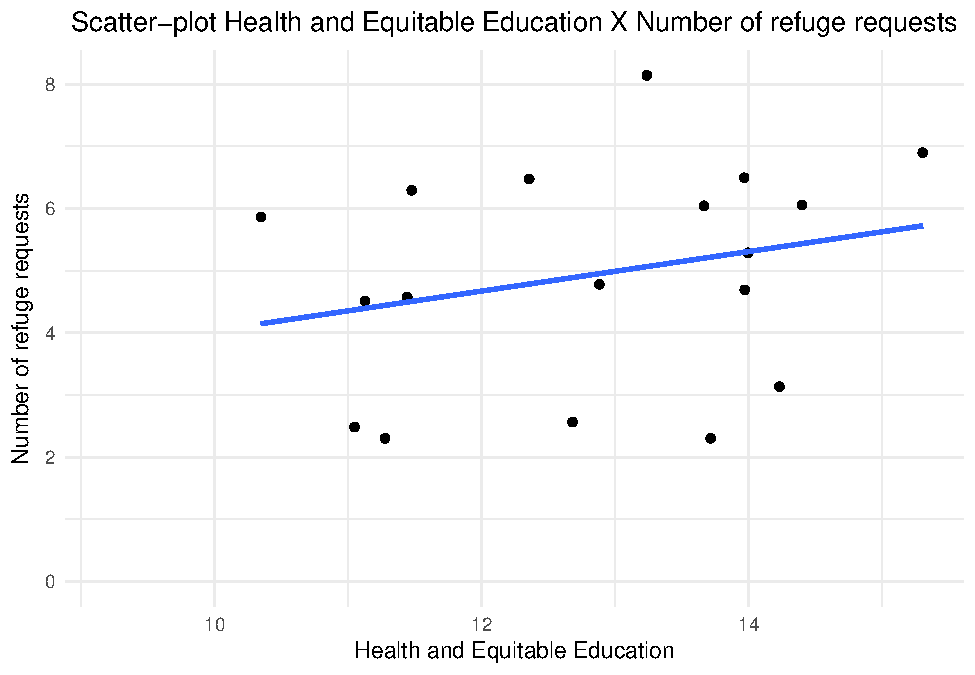
\includegraphics{stephanie-moura-rmarkdown-tf-ad-ufpe-2018_files/figure-latex/model_1_2-1.pdf}

Concerning the graphic that associates the variables ``number of refuge
requests'' and ``public services'', we can see that as public services
increase, the number of requests for refuge decreases, in 2015,
following the same pattern as the 2011's results.

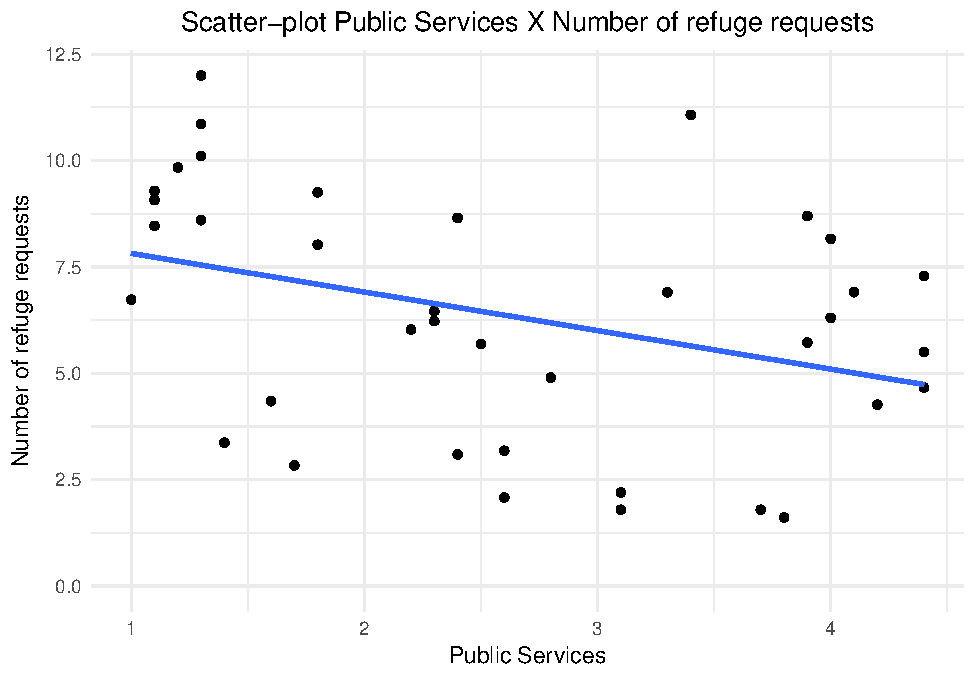
\includegraphics{stephanie-moura-rmarkdown-tf-ad-ufpe-2018_files/figure-latex/model_1_3-1.pdf}

Concerning the graph that associates the variables ``number of refuge
requests'' and ``Health and equitable education'', we can see that as
the Health and Equitable education index increases, the number of
refugee requests increases, in 2015, following the same pattern of
results of 2011.

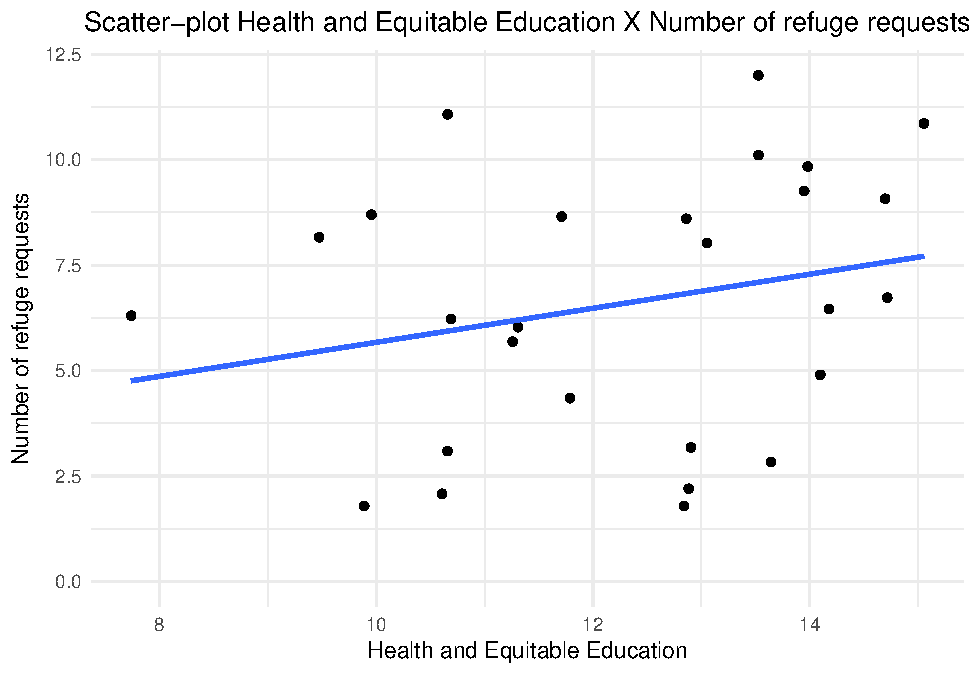
\includegraphics{stephanie-moura-rmarkdown-tf-ad-ufpe-2018_files/figure-latex/model_1_4-1.pdf}

In association graphs, we can not find nonlinear relationships.
Therefore, we will carry out the analyzes without including polynomials
in the models.

Variable's description table

\begin{longtable}[]{@{}ll@{}}
\toprule
Variable code & Variable name\tabularnewline
\midrule
\endhead
Applied & Number of refuge requests\tabularnewline
ffp\_ps & Public Services\tabularnewline
bs\_ee & Equitable Education\tabularnewline
bs\_h & Health\tabularnewline
fh\_pr & Political Rights\tabularnewline
\bottomrule
\end{longtable}

\emph{source: own elaboration}

\section{Results}\label{results}

To answer the research question, we used 4 multiple linear regression
models, alternating the independent variables of the model and the
analyzed years.

Regarding the first model, which refers to the year 2011, with the
dependent variable LogApplied, the independent Public Services and the
control variable Political Rights. The variable Public Services had a
negative effect on the application of requests for refugees from Syrians
in the countries analyzed. The p-value was very close to the 5\%
threshold. The control variable Political Rights did not present
statistical significance in the model. The r2 of the model presented a
median magnitude, since it revealed a prediction capacity of 10\% of the
variance of the dependent variable.

\begin{table}[!htbp] \centering 
  \caption{Resultados do Modelo 1} 
  \label{} 
\begin{tabular}{@{\extracolsep{5pt}}lc} 
\\[-1.8ex]\hline \\[-1.8ex] 
\\[-1.8ex] & LogApplied \\ 
\hline \\[-1.8ex] 
 ffp\_ps & $-$0.932$^{*}$ \\ 
  & (0.459) \\ 
  fh\_pr & 0.220 \\ 
  & (0.437) \\ 
  Constant & 6.483$^{***}$ \\ 
  & (1.062) \\ 
 N & 33 \\ 
R$^{2}$ & 0.157 \\ 
Adjusted R$^{2}$ & 0.100 \\ 
Residual Std. Error & 1.977 (df = 30) \\ 
F Statistic & 2.784$^{*}$ (df = 2; 30) \\ 
\hline \\[-1.8ex] 
\multicolumn{2}{l}{$^{*}$p $<$ .1; $^{**}$p $<$ .05; $^{***}$p $<$ .01} \\ 
\end{tabular} 
\end{table}

As for the second model, which refers to the year 2011, with the
dependent variable LogApplied, and the independent Equitable Education
and Health, in addition to the control variable, Political Rights, it is
noteworthy that in this model 2, none of the variables had a significant
effect. This is also reflected in the r2 of the model, which is close to
zero.

\begin{table}[!htbp] \centering 
  \caption{Resultados do Modelo 2} 
  \label{} 
\begin{tabular}{@{\extracolsep{5pt}}lc} 
\\[-1.8ex]\hline \\[-1.8ex] 
\\[-1.8ex] & LogApplied \\ 
\hline \\[-1.8ex] 
 bs\_ee & 0.069 \\ 
  & (0.596) \\ 
  bs\_h & 0.669 \\ 
  & (0.405) \\ 
  fh\_pr & 1.652 \\ 
  & (2.145) \\ 
  Constant & $-$1.836 \\ 
  & (5.945) \\ 
 N & 18 \\ 
R$^{2}$ & 0.178 \\ 
Adjusted R$^{2}$ & 0.002 \\ 
Residual Std. Error & 1.770 (df = 14) \\ 
F Statistic & 1.012 (df = 3; 14) \\ 
\hline \\[-1.8ex] 
\multicolumn{2}{l}{$^{*}$p $<$ .1; $^{**}$p $<$ .05; $^{***}$p $<$ .01} \\ 
\end{tabular} 
\end{table}

The third model refers to the year 2015, with the dependent variable
LogApplied, and the independent Public Services, in addition to the
control variable, Political Rights. It is notable that in this model 3,
the variable Public Services presented a negative and significant effect
and the variable Political Rights did not present statistical
significance. Compared with model 1, which includes the same variables,
but for the year 2011, the variable Public Services had its negative
effect accentuated, and the r2 of the model became more expressive.

\begin{table}[!htbp] \centering 
  \caption{Model 3} 
  \label{} 
\begin{tabular}{@{\extracolsep{5pt}}lc} 
\\[-1.8ex]\hline \\[-1.8ex] 
\\[-1.8ex] & LogApplied \\ 
\hline \\[-1.8ex] 
 ffp\_ps & $-$1.331$^{**}$ \\ 
  & (0.543) \\ 
  fh\_pr & 0.493 \\ 
  & (0.440) \\ 
  Constant & 8.958$^{***}$ \\ 
  & (1.123) \\ 
 N & 38 \\ 
R$^{2}$ & 0.161 \\ 
Adjusted R$^{2}$ & 0.113 \\ 
Residual Std. Error & 2.726 (df = 35) \\ 
F Statistic & 3.347$^{**}$ (df = 2; 35) \\ 
\hline \\[-1.8ex] 
\multicolumn{2}{l}{$^{*}$p $<$ .1; $^{**}$p $<$ .05; $^{***}$p $<$ .01} \\ 
\end{tabular} 
\end{table}

The fourth model is the one that presented the greatest explanatory
capacity of the variance of the dependent variable. It concerns the year
2015, with the dependent variable LogApplied, and the independent
variables Equitable Education and Health, in addition to the control
variable, Political Rights. In the fourth model, the independent
variable Health and the control variable Political Rights presented
positive and significant effects. The variable Equitable Education did
not present statistical significance.

\begin{table}[!htbp] \centering 
  \caption{Model 4} 
  \label{} 
\begin{tabular}{@{\extracolsep{5pt}}lc} 
\\[-1.8ex]\hline \\[-1.8ex] 
\\[-1.8ex] & LogApplied \\ 
\hline \\[-1.8ex] 
 bs\_ee & 0.069 \\ 
  & (0.596) \\ 
  bs\_h & 0.669 \\ 
  & (0.405) \\ 
  fh\_pr & 1.652 \\ 
  & (2.145) \\ 
  Constant & $-$1.836 \\ 
  & (5.945) \\ 
 N & 18 \\ 
R$^{2}$ & 0.178 \\ 
Adjusted R$^{2}$ & 0.002 \\ 
Residual Std. Error & 1.770 (df = 14) \\ 
F Statistic & 1.012 (df = 3; 14) \\ 
\hline \\[-1.8ex] 
\multicolumn{2}{l}{$^{*}$p $<$ .1; $^{**}$p $<$ .05; $^{***}$p $<$ .01} \\ 
\end{tabular} 
\end{table}

A summary of the four models analyzed is presented below. From it it is
possible to see significant fluctuations in the effect of the variable
Equitable Education; a relation that suggests that the control variable
Political Rights has greater effect on th

\begin{table}[!htbp] \centering 
  \caption{Models Results} 
  \label{} 
\begin{tabular}{@{\extracolsep{5pt}}lcc} 
\\[-1.8ex]\hline \\[-1.8ex] 
\\[-1.8ex] & \multicolumn{2}{c}{LogApplied} \\ 
 & Model 1 & Model 2 \\ 
\hline \\[-1.8ex] 
 ffp\_ps & $-$0.932$^{*}$ &  \\ 
  & (0.459) &  \\ 
  bs\_ee &  & 0.069 \\ 
  &  & (0.596) \\ 
  bs\_h &  & 0.669 \\ 
  &  & (0.405) \\ 
  fh\_pr & 0.220 & 1.652 \\ 
  & (0.437) & (2.145) \\ 
  Constant & 6.483$^{***}$ & $-$1.836 \\ 
  & (1.062) & (5.945) \\ 
 N & 33 & 18 \\ 
R$^{2}$ & 0.157 & 0.178 \\ 
Adjusted R$^{2}$ & 0.100 & 0.002 \\ 
Residual Std. Error & 1.977 (df = 30) & 1.770 (df = 14) \\ 
F Statistic & 2.784$^{*}$ (df = 2; 30) & 1.012 (df = 3; 14) \\ 
\hline \\[-1.8ex] 
\multicolumn{3}{l}{$^{*}$p $<$ .1; $^{**}$p $<$ .05; $^{***}$p $<$ .01} \\ 
\end{tabular} 
\end{table}

\begin{table}[!htbp] \centering 
  \caption{Models Results} 
  \label{} 
\begin{tabular}{@{\extracolsep{5pt}}lcc} 
\\[-1.8ex]\hline \\[-1.8ex] 
\\[-1.8ex] & \multicolumn{2}{c}{LogApplied} \\ 
 & Model 3 & Model 4 \\ 
\hline \\[-1.8ex] 
 ffp\_ps & $-$1.331$^{**}$ &  \\ 
  & (0.543) &  \\ 
  bs\_ee &  & $-$0.032 \\ 
  &  & (0.477) \\ 
  bs\_h &  & 2.226$^{***}$ \\ 
  &  & (0.502) \\ 
  fh\_pr & 0.493 & 6.326$^{***}$ \\ 
  & (0.440) & (1.810) \\ 
  Constant & 8.958$^{***}$ & $-$14.393$^{**}$ \\ 
  & (1.123) & (6.097) \\ 
 N & 38 & 27 \\ 
R$^{2}$ & 0.161 & 0.468 \\ 
Adjusted R$^{2}$ & 0.113 & 0.398 \\ 
Residual Std. Error & 2.726 (df = 35) & 2.424 (df = 23) \\ 
F Statistic & 3.347$^{**}$ (df = 2; 35) & 6.739$^{***}$ (df = 3; 23) \\ 
\hline \\[-1.8ex] 
\multicolumn{3}{l}{$^{*}$p $<$ .1; $^{**}$p $<$ .05; $^{***}$p $<$ .01} \\ 
\end{tabular} 
\end{table}

\section{Assumptions}\label{assumptions}

After the data results, it's possible to realize that the data is
homocedastic since there is no pattern visible in the dispersion of the
error. When the histogram of the descriptive statistics is made, such as
it's summary, it's possible to realize that most of the cases are on the
left, near zero, with some outliers. This can be proved with the summary
at the analysis, where is possible to realize that the 1st. qu and
median are on numbers way below the mean and the others quarters. When
the log enters on the analysis, it's possible to realize that the
differences are smaller and the universe of analysis os smaller as well.
With this proof, the variabel is transformed into log. After that, a
descriptive summary is made for each variable on the model, followed by
an histogram. On the Equitable Education summary, it's possible to
visualize that the rates maximum are 7.855 out of 10, and most of the
cases are between the mean and the maximum, indicating that the
equitable education in the analyzed countries are show good rates, above
the mean. When the Health is the variable analyzed, it's possible to
percieve that, just like the Equitable Education summary, this summary
shows that most of the cases are also above the mean. When Public
Services are analyzed, the results show the same tendency as the two
prior variables. However, when the Political Rights is the variable
analyzed, the tendency is that the cases are concentrated on ``1'' than
on ``7'', which shows that the analyzed countries are free when the
topic referred is political rights.

Then, separate databases are created by year, such as the models used in
this paper. The first model has the variables Political Rights and
Public Services referred to the number of refuge requests in 2011. The
second model has the variables Equitable Education, Health and Political
Rights referred to the number of refuge requests in 2011. The third
model has the variables Political Rights and Public Services referred to
the number of refuge requests in 2015. The fourth model has the
variables Equitable Education, Health and Political Rights referred to
the number of refuge requests in 2015.

\begin{itemize}
\tightlist
\item
  Checking the residuals normality: Below you can see the histograms of
  the residuals of the four models. We did not identify deviations of
  normality in the distribution of residues and all of them presented
  approximate mean zero.
\end{itemize}

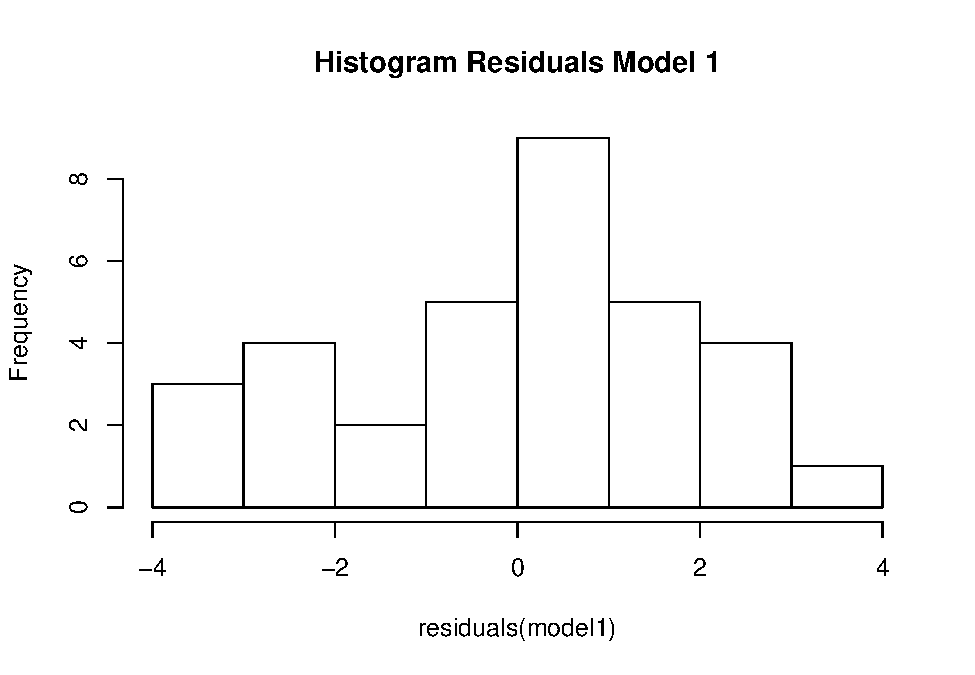
\includegraphics{stephanie-moura-rmarkdown-tf-ad-ufpe-2018_files/figure-latex/ggplot_resmodel_1-1.pdf}

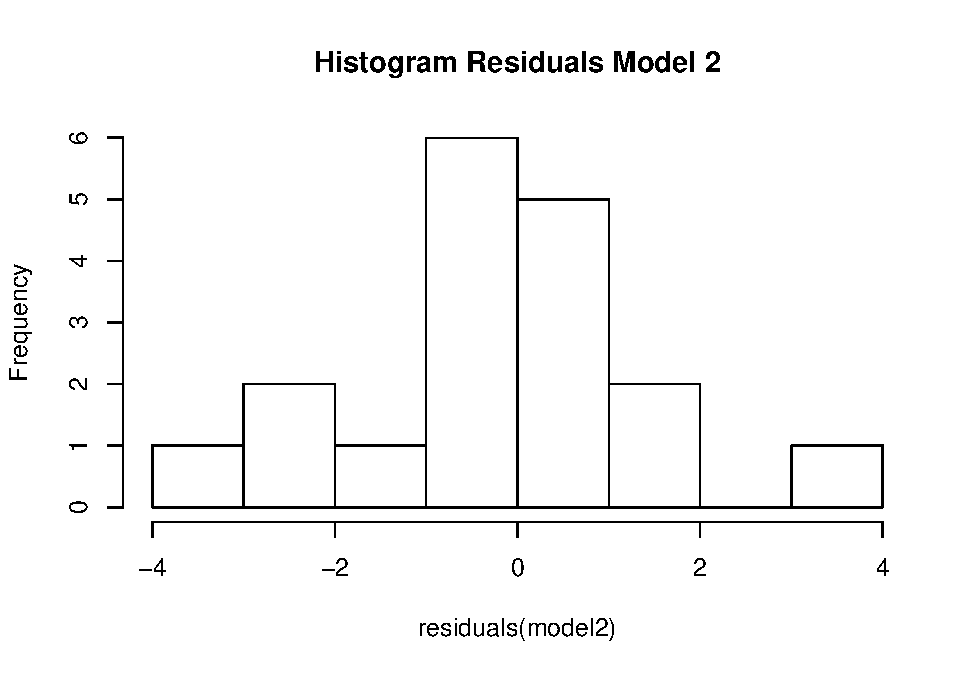
\includegraphics{stephanie-moura-rmarkdown-tf-ad-ufpe-2018_files/figure-latex/ggplot_resmodel_2-1.pdf}

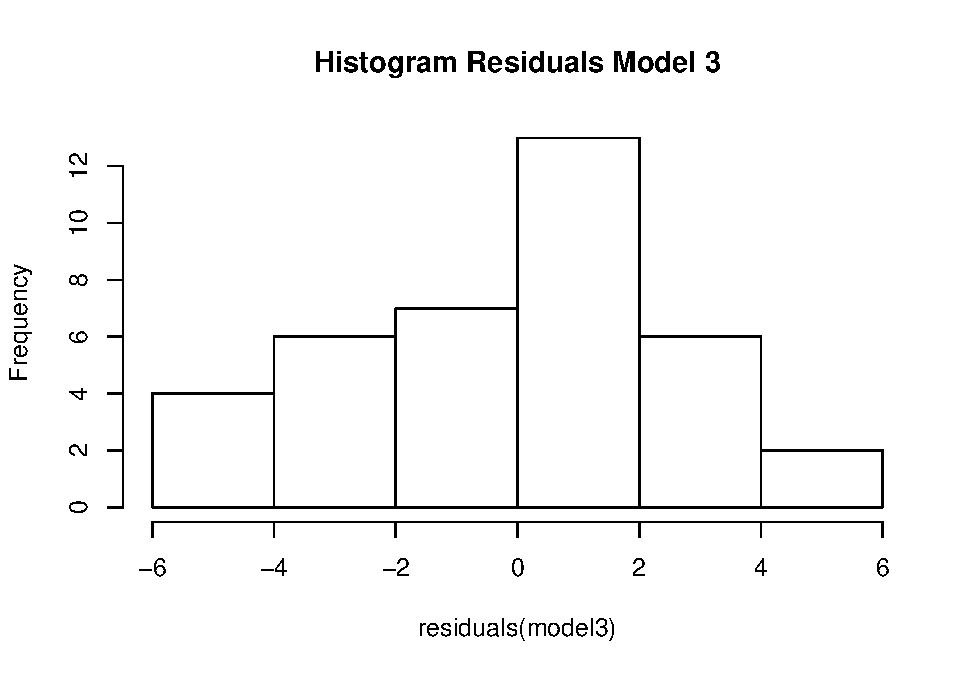
\includegraphics{stephanie-moura-rmarkdown-tf-ad-ufpe-2018_files/figure-latex/ggplot_resmodel_3-1.pdf}

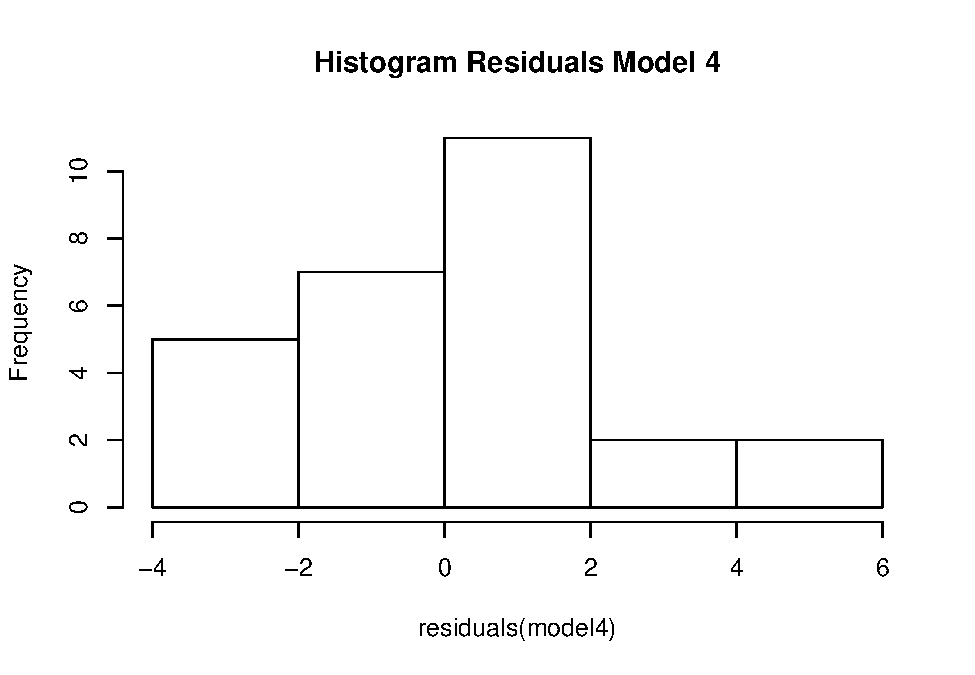
\includegraphics{stephanie-moura-rmarkdown-tf-ad-ufpe-2018_files/figure-latex/ggplot_resmodel_4-1.pdf}

\begin{itemize}
\tightlist
\item
  Checking heteroskedasticity: In the following figures, it is possible
  to visualize the graphs of the predicted values versus residuals of
  the four models. In none of them can we identify extreme values that
  would be indicative of the presence of heteroscedasticity.
\end{itemize}

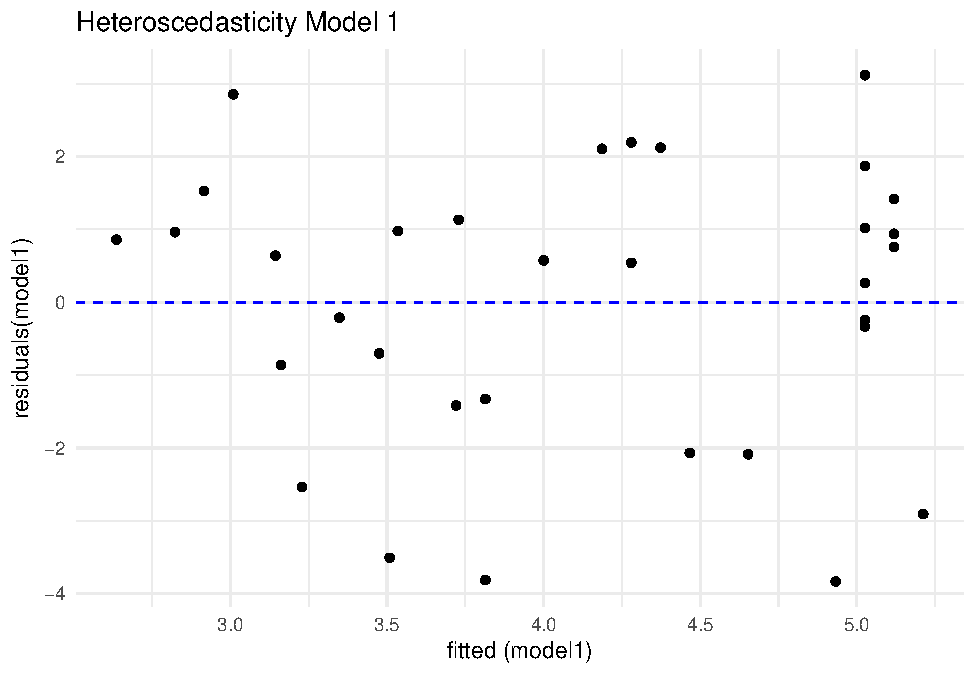
\includegraphics{stephanie-moura-rmarkdown-tf-ad-ufpe-2018_files/figure-latex/ggplot_model_1-1.pdf}

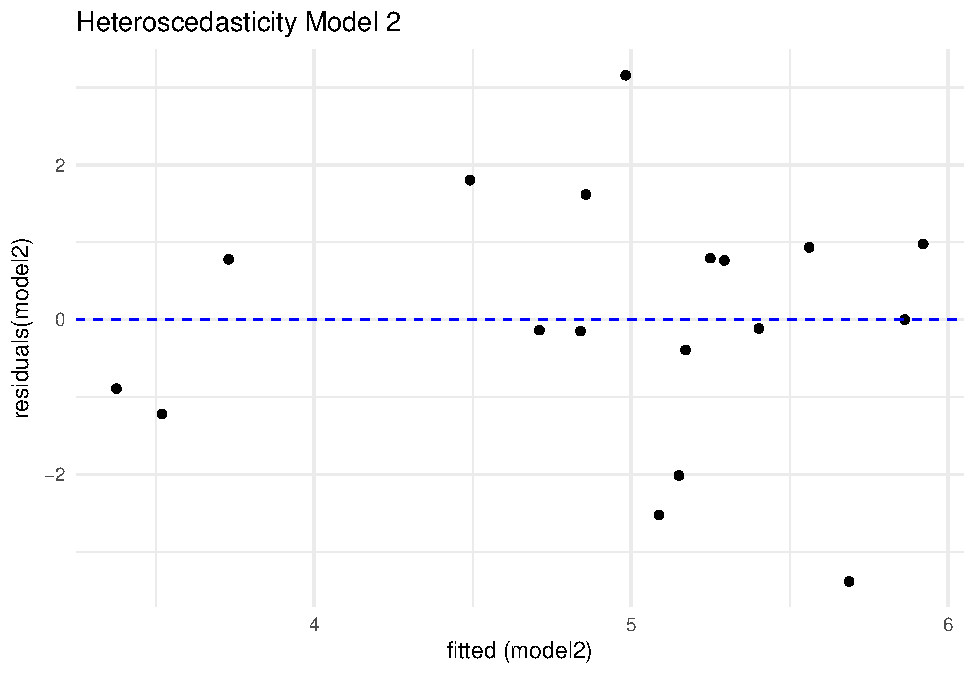
\includegraphics{stephanie-moura-rmarkdown-tf-ad-ufpe-2018_files/figure-latex/ggplot_model_2-1.pdf}

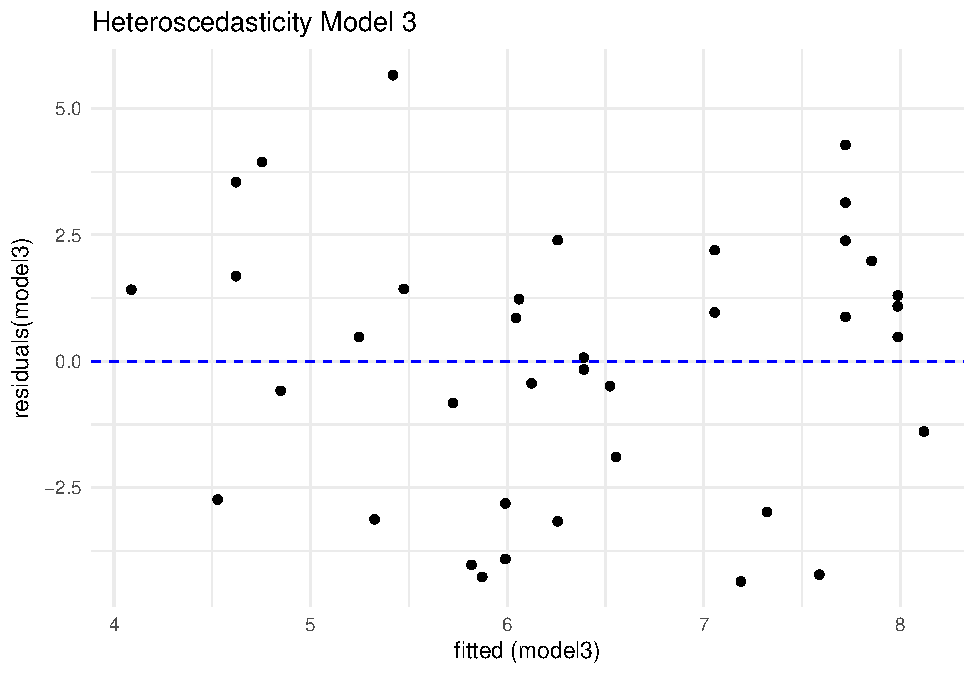
\includegraphics{stephanie-moura-rmarkdown-tf-ad-ufpe-2018_files/figure-latex/ggplot_model_3-1.pdf}

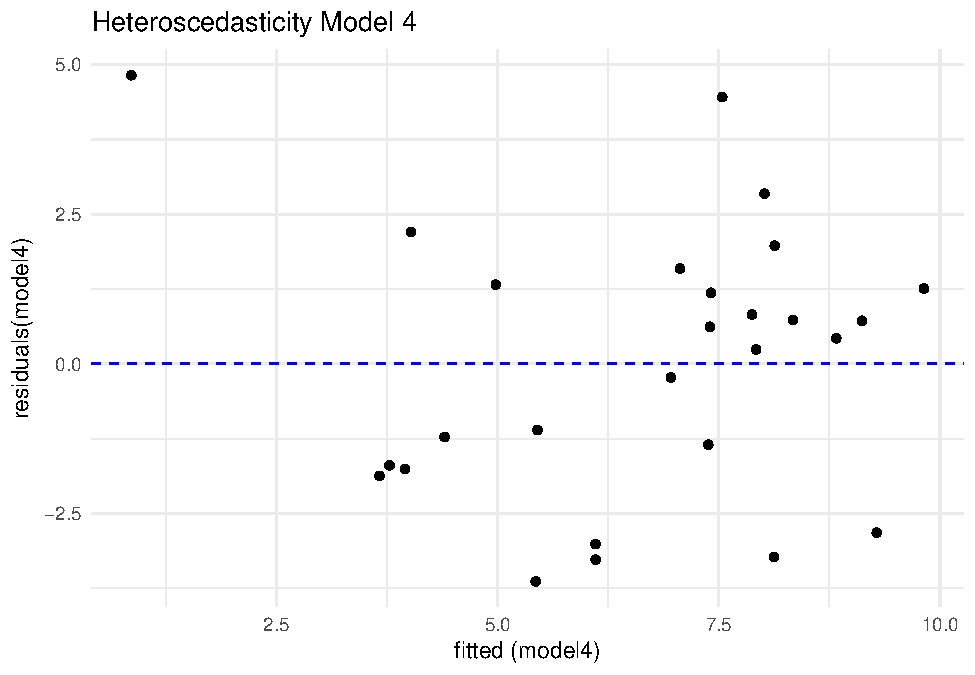
\includegraphics{stephanie-moura-rmarkdown-tf-ad-ufpe-2018_files/figure-latex/ggplot_model_4-1.pdf}

\begin{itemize}
\tightlist
\item
  Checking multicolinearity: Below it is possible to visualize the
  coefficients of inflation of the variance of the variables in the four
  models. None of the coefficients presented values higher than 7,
  indicating that we did not find evidence of presence of
  multicollinearity in the models.
\end{itemize}

\begin{verbatim}
##   ffp_ps    fh_pr 
## 1.866647 1.866647
\end{verbatim}

\begin{verbatim}
##    bs_ee     bs_h    fh_pr 
## 1.356414 1.033322 1.386391
\end{verbatim}

\begin{verbatim}
##   ffp_ps    fh_pr 
## 1.946842 1.946842
\end{verbatim}

\begin{verbatim}
##    bs_ee     bs_h    fh_pr 
## 1.119219 2.110542 2.271114
\end{verbatim}

\section{Conclusion}\label{conclusion}

Responding to the research question, it is notable that the variable
``Public Services'' was contrary to expectations when used as a Welfare
State index, with a negative effect on the number of asylum applications
of Syrian refugees in the European countries analyzed. In 2015, the
negative effect was even more significant for this variable compared to
2011. Corroborating this result, equity in education also had no effect
on the number of asylum applications, either in 2011 or 2015. On the
other hand, the Health variable presented ambiguous results, not being
significant in 2011, but having a positive and significant effect in
2015. The work hypothesis was falsified, since, with the variables
analyzed, no evidence was found of a positive relationship between the
Welfare State and the number of asylum requests for Syrian refugees in
European countries

\section*{References}\label{references}
\addcontentsline{toc}{section}{References}

\hypertarget{refs}{}
\hypertarget{ref-briggs}{}
Briggs, Asa. 1961. ``The Welfare State in Historical Perspective'' 2
(2). Archives Européennes de Sociologie: 221--58.
doi:\href{https://doi.org/https://doi.org/10.1017/S0003975600000412}{https://doi.org/10.1017/S0003975600000412}.

\hypertarget{ref-leneide}{}
Duarte-Plon, Leneide. 2015. ``Imigração E Refugiados Na Europa - O
Desafio Do Século,'' August.
\url{https://www.cartamaior.com.br/?/Editoria/Internacional/Imigracao-e-refugiados-na-Europa-O-desafio-do-seculo/6/34349}.

\hypertarget{ref-marshall}{}
Marshall, Thomas Humphrey. 1992. ``Citizenship and Social Class.'' Pluto
Press.

\hypertarget{ref-franstimmermans}{}
Timmermans, Frans. 2018. ``Speech by First Vice-President Frans
Timmermans at the European Parliament Plenary Session on the Preparation
of the European Council Meeting of 28 and 29 June 2018,'' June. European
Commission.
\url{http://europa.eu/rapid/press-release_SPEECH-18-4142_en.htm}.

\end{document}


